\section{Formula Visualization and Verbalization}
\label{sec:verbviz}
Episodic Logic formulas are difficult for untrained readers to make sense of; they contain various non-lexical symbols and frequently split into several smaller formulas. However, the predicate-argument structure and semantic types of ELFs are still designed to closely mirror surface-form English, modulo some ``elbow grease'' expended for transduction. In this section, we describe two means of visualizing EL formulas to enable untrained evaluators to interpret their meaning in our quality experiments: tabular representations and GPT-driven verbalizations.

\subsection{Tabular Representations}

For each step and goal formula in each learned schema, we first constructed a \textit{tabular representation} (tabrep), meant to render the EL formula in a human-readable way while still illustrating its formal predicate-argument structure. Two examples of tabreps can be seen in Figure~\ref{fig:goal_eval_eg}, which contains representations of the formulas \el{(?X (WANT.V (KA (FIND.V ?B))))} and \el{(?X ((ADV-A (FOR.P ?B)) LOOK.V))}, with context role type formulas \el{(?X PERSON.N)} and \el{(?B BOOK.N)}. Each tabrep has slots for \texttt{arg0}, the prefix argument; \texttt{action}, the verb predicate; \texttt{adv}, for single adverbial modifiers derived from monadic prepositional predicates; and \texttt{arg1} and \texttt{arg2}, for up to two postfix verb arguments. Arguments in tabreps can also recursively nest other tabreps, such as in the first (top) example in in Figure~\ref{fig:goal_eval_eg}; because tabreps represent actions or events, they must be reified to act as arguments, and thus the reifier (\texttt{TO}, a.k.a. \el{KA}, in the example) is represented in the \texttt{rei} slot of any nested tabrep. Leaf-level tabrep slot fillers are single words derived either from the lexical form of the verb or preposition predicate, or the first noun type predicate for the individual as found in the context formulas.

\begin{figure}
    \centering
    {
    \setlength{\fboxsep}{2pt}
    \definecolor{tabrepgray}{HTML}{DDDDDD}
    \fcolorbox{black}{tabrepgray}{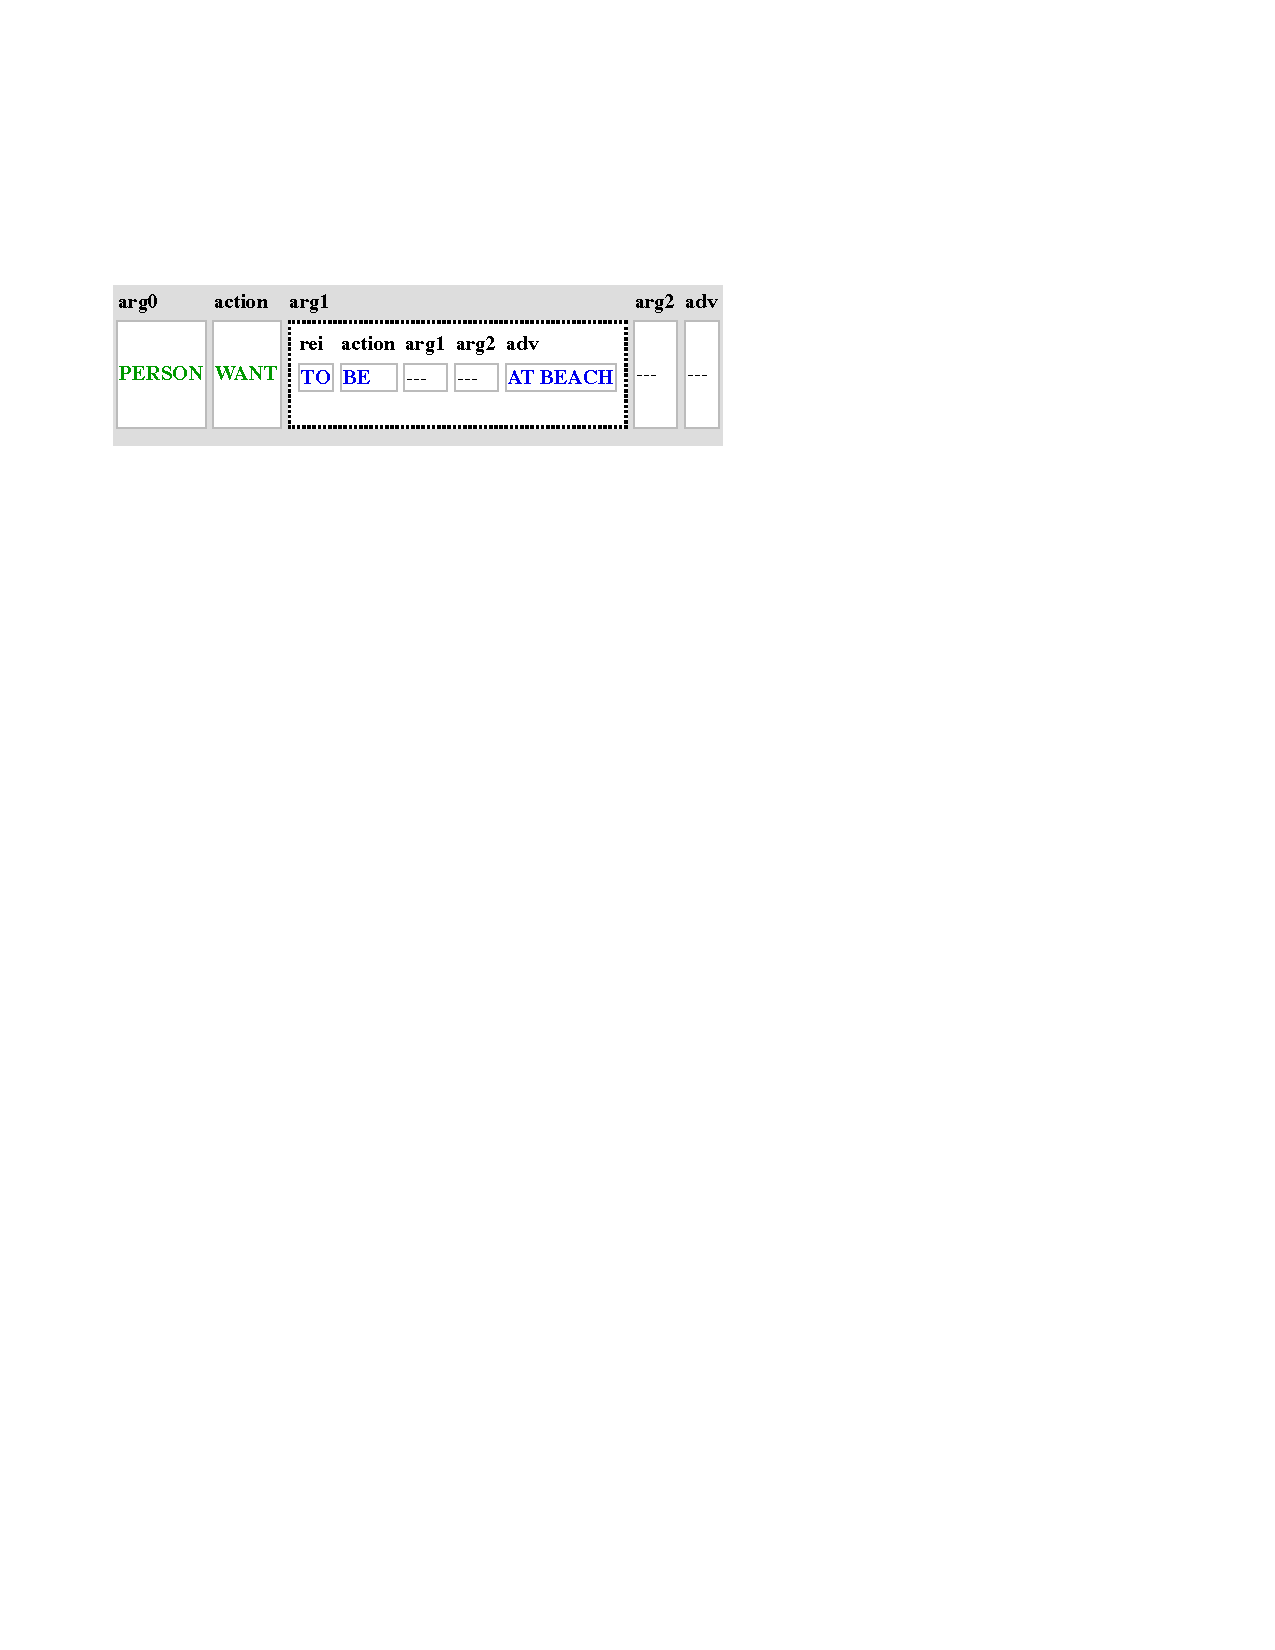
\includegraphics{CH5_eval/tabrep.pdf}}
    }
    \caption{A tabular representation (tabrep) of the ELF $\exists$ \el{X(X PERSON.N) .} $\exists$ \el{B(B BEACH.N)} \texttt{. (X (WANT.V (KA ((ADV-A (AT.P B)) BE.V))))}. This tabrep exhibits a nested structure, with the first argument to the predicate \el{WANT.V} being a tabrep of a kind of action.}
    \label{fig:tabrep}
\end{figure}

Left-to-right linearizations of nested tabreps are designed to be interpretable by untrained evaluators as crude English sentences while still illustrating the recursive structure of EL formulas. However, further refinement of the tabrep verbalizations into more fluent English is possible, as we show in Section~\ref{sec:gpt-reverb}.

\subsection{GPT Verbalizations}
\label{sec:gpt-reverb}
To more fluently verbalize schema ELFs, we first apply rule-based transductions to serialize each formula's lexical EL predicates into pseudo-English representations. This ``crude'' verbalizer replaces entities in a set of ELFs with descriptions formed from their atemporal type constraints, i.e. noun and adjective predications. The first such replacement is introduced with an indefinite article, while all subsequent replacements use the definite article. An example of this can be seen in the ``Symbolic Verbalization'' row of Table~\ref{tab:gpt_reverb}. When multiple entities of the same type are introduced in the ELFs, the articles are modified to indicate identity numerically: ``\textit{an X}'' becomes ``\textit{a second X}'', and so on. Plural operators are applied to noun predicates to form plural nouns, and adverbial modifiers are appended to the end of the linearized predicate-argument structure. Complex terms and adverbials are recursively processed. Verbs are also pluralized or singularized in accordance with the plurality of the subject, e.g. ``\textit{a mother \textbf{feeds} the baby}'' and ``\textit{some mothers \textbf{feed} the baby}''.

This pseudo-English is crude and often unappealing, or even illegible, to untrained observers. However, having performed the appropriate variable de-referencing and ``flattening'', all information needed to interpret the sentence is now, in principle, linearized into one representation. With this in mind, we cast the problem of refinement of these crude verbalizations into fluent English as one of \textit{translation}, and turn to pre-trained transformer language models as a base for the solution of this translation problem.

\begin{table}[ht]
    \centering
    \begin{tabular}{l|l}
       \textsc{English} & A mother feeds her babies. \\
       \hline
       \textsc{ELF (conjunctive)} & \el{(\textbf{?M} (FEED.V \textbf{?B}))} $\land$ \\
         & \el{(\textbf{?M} MOTHER.N)} $\land$ \\
         & \el{(\textbf{?B} (PLUR BABY.N))} $\land$ \\
         & \el{(\textbf{?B} (PERTAIN-TO \textbf{?M}))} \\
         \hline
       \textsc{Symbolic Verbalization} & $\underbrace{\text{A MOTHER}}_{\textbf{\el{?M}}}$ FEEDS $\overbrace{\text{THE BABIES OF} \underbrace{\text{THE MOTHER}}_{\textbf{\el{?M}}}}^{\textbf{\el{?B}}}$ \\
       \hline
       \textsc{GPT-2 Re-Verbalization} & A mother feeds her babies.
    \end{tabular}
    \caption{An illustration of an English sentence, its ELF parse, the crude symbolic verbalization of the parse, and a GPT-2 re-verbalization of that crude verbalization.}
    \label{tab:gpt_reverb}
\end{table}

For each of 3,783 sentences derived from 913 stories generated by GPT-J 6B\footnote{20 stories were generated for each of 50 topics not used for the generation of schemas in the experiment. Empty stories and unparseable sentences were discarded, leaving 913 stories and 3,783 sentences.}, we parsed ELFs and derived crude verbalizations. Like in the \texttt{ulf-gpt2} project detailed in Section~\ref{sec:ulf-gpt2}, we then created pairs of the form \begin{center}
\texttt{THIS IS EXAMPLE \textbf{<SEP>} This is an example. \textbf{<END>}}
\end{center}
for the crude and natural versions of each sentence and fine-tuned a \texttt{gpt2-large} model on the corresponding set of pairs. The crude sentence comes first due to the autoregressive nature of the language model. The resulting fine-tuned language model can be used to create more fluent English verbalizations of the ELFs evaluated in the study. An example of a fluent sentence, computed from a tabrep by the language model, is shown in the evaluation form in Figure~\ref{fig:gpt_step_eval_eg}; its corresponding tabrep is shown in the form in Figure~\ref{fig:step_eval_eg}.